
\section{The Main Upper Bound}\label{sec:main-upper}

In this section we prove the paper's headline upper bound
\[
  \L(n) \le \left(\frac{\Wfour}{2}+o(1)\right)n < 0.19n.
\]
The proof uses the following explicit strategy.  Shortener plays the smallest legal odd prime for a long initial prefix of
\[
  K = \left\lfloor \frac{(1-\eps)n}{2\log n}\right\rfloor
\]
turns.  This prefix is available for all sufficiently large $n$.

\begin{lemma}[Existence of the odd-prime prefix]\label{lem:prefix-existence}
Fix $0<\eps<1$ and
\[
  K=\left\lfloor \frac{(1-\eps)n}{2\log n}\right\rfloor.
\]
For all sufficiently large $n$, before each of Shortener's first $K$ turns
there is a legal odd prime.  Hence the smallest-legal-odd-prime strategy can
be followed for a prefix of $K$ Shortener moves.
\end{lemma}

\begin{proof}
Since the board is $\{2,3,\ldots,n\}$, no legal move equals $1$.
Consider the moment before Shortener's $j$th move in this prefix, with
$1\le j\le K$.  At most $2j-1$ previous moves have occurred.  A previous move
$x\le n$ can make at most one odd prime $p>\sqrt n$ illegal: if two such
primes divided $x$, then $x>n$, while the only other way for $x$ to be
comparable with such a prime is $x=p$ itself.  Thus at most $2j-1$ odd primes
in $(\sqrt n,n]$ have been made illegal.

By the prime number theorem,
\[
  \pi(n)-\pi(\sqrt n)\sim \frac{n}{\log n}>2K
\]
for all sufficiently large $n$.  Since $2j-1<2K$, at least one odd prime
$p\in(\sqrt n,n]$ remains legal before Shortener's $j$th prefix move.  In
particular the game has not ended, and Shortener's rule has a legal odd prime
to play.
\end{proof}

Let
\[
  q_1 < q_2 < \cdots < q_K
\]
be the odd primes she plays during that prefix.  The argument has four layers:
\begin{enumerate}
  \item a one-sided lower-profile estimate for the counting function of the $q_j$;
  \item a monotone envelope and inversion producing a comparison sequence
    $b_j \ge q_j$ with explicit moment limits;
  \item a fourth-order Bonferroni comparison theorem for arbitrary increasing
    odd-prime comparison sequences;
  \item a prime-rounding bridge that replaces the real sequence $b_j$ by actual
    odd primes $p_j$, using the key half-density slack supplied by the
    prime-rounding bridge of \Cref{thm:prime-bridge}.
\end{enumerate}

\begin{sloppypar}
The assembly from \Cref{lem:right-continuous-cumulative-envelope} through
\Cref{lem:exceptional-mass-cutoff-discrepancy} is the longest prose stretch
in the paper and the part most sensitive to auditing.  Its arithmetic
kernels---envelope properties and flat-block mass estimates---have
zero-sorry Lean artifacts in the files \texttt{Envelope.lean} and
\texttt{FlatMass.lean} of the \texttt{Round15Bonferroni4} project; the
assembly itself is prose, with the moment-convergence hypotheses feeding
the zero-sorry endgame reduction in \texttt{Target.lean}.
\end{sloppypar}

\subsection{A lower-profile envelope for Shortener's primes}

Write
\[
  S_K(X) := \#\{j\le K : q_j \le X\},
  \qquad
  u := \frac{\log X}{\log n}.
\]
We establish a one-sided lower envelope for the counting function of
Shortener's captured primes.  On the interval
\[
  u \in \left(\frac{1}{h+1},\frac1h\right],
\]
the lower-profile function is
\[
  \rhoU(u) = \frac{1}{(\lfloor 1/u \rfloor+1)u} = \frac{1}{(h+1)u}.
\]
\Cref{fig:lower-profile} plots this piecewise-hyperbolic profile on $(0, 1]$.

\begin{figure}[!htbp]
\centering
\begin{tikzpicture}
\begin{axis}[
    width=0.85\textwidth,
    height=5.5cm,
    xmin=0.12, xmax=1.02,
    ymin=0, ymax=1.1,
    xlabel={$u = \log X / \log n$},
    ylabel={$\rho(u)$},
    xtick={0.1667, 0.2, 0.25, 0.3333, 0.5, 1},
    xticklabels={$\tfrac{1}{6}$, $\tfrac{1}{5}$, $\tfrac{1}{4}$, $\tfrac{1}{3}$, $\tfrac{1}{2}$, $1$},
    ytick={0.5, 0.6667, 0.75, 1},
    yticklabels={$\tfrac{1}{2}$, $\tfrac{2}{3}$, $\tfrac{3}{4}$, $1$},
    axis lines=left,
    tick label style={font=\scriptsize},
    label style={font=\small},
    every axis plot/.append style={very thick, blue}
]
  % Piece h=1 on (1/2, 1]: rho(u) = 1/(2u)
  \addplot[domain=0.5:1, samples=80] {1/(2*x)};
  % Piece h=2 on (1/3, 1/2]: rho(u) = 1/(3u)
  \addplot[domain=0.3334:0.5, samples=80] {1/(3*x)};
  % Piece h=3 on (1/4, 1/3]: rho(u) = 1/(4u)
  \addplot[domain=0.2501:0.3333, samples=80] {1/(4*x)};
  % Piece h=4 on (1/5, 1/4]: rho(u) = 1/(5u)
  \addplot[domain=0.2001:0.25, samples=80] {1/(5*x)};
  % Piece h=5 on (1/6, 1/5]: rho(u) = 1/(6u)
  \addplot[domain=0.1667:0.2, samples=80] {1/(6*x)};

  % Vertical discontinuity markers (dotted) at each breakpoint
  \foreach \b in {0.5, 0.3333, 0.25, 0.2} {
    \addplot[dotted, gray, forget plot] coordinates {(\b, 0) (\b, 1)};
  }
\end{axis}
\end{tikzpicture}
\caption{The lower-profile function $\rho(u) = 1/((\lfloor 1/u\rfloor+1)u)$ on
$(0, 1]$. On each interval $(1/(h+1), 1/h]$ with $h \ge 1$, $\rho$ is the
strictly decreasing hyperbola $u \mapsto 1/((h+1)u)$, jumping up to $1$ at
each left endpoint $u = 1/(h+1)^+$ and descending to $h/(h+1)$ at $u = 1/h$.
The monotone right-continuous cumulative envelope built in
\Cref{lem:right-continuous-cumulative-envelope} and inverted in
\Cref{lem:generalized-inverse-comparison} is derived from this profile.}
\label{fig:lower-profile}
\end{figure}

\begin{lemma}[Local prime-count per range]\label{lem:prime-count-per-range}
Let Shortener follow the smallest-legal-odd-prime strategy.  Fix an integer
$h\ge1$ and real numbers $2\le Y<X\le n$ with
\[
  Y^{h+1}>n.
\]
Assume the odd-prime strategy is available until the first time her next
odd-prime move would exceed $X$, and let $S(X)$ be the number of odd primes at
most $X$ which Shortener has played by that stopping time.  Then
\[
  S(X)\ge\frac{\pi(X)-\pi(Y)}{h+1}-O_h(1).
\]
In particular, if $n^{1/(h+1)}<Y<X\le n^{1/h}$, then every prime
$p\in(Y,X]$ lies in the packet regime $p^h\le n<p^{h+1}$ and the same lower
bound holds.
\end{lemma}

\begin{proof}
Shortener's odd-prime moves are increasing: once a prime has become illegal it
cannot become legal later, and the strategy always chooses the smallest legal
odd prime.  At the stopping time in the definition of $S(X)$, no odd prime
$p\le X$ is still legal.  Therefore every odd prime $p\in(Y,X]$ has one of two
forms: either Shortener herself has played $p$, or some earlier Prolonger move
was divisible by $p$.

Let
\[
  M:=\#\{p\in\PP:\ Y<p\le X,\ p\text{ odd}\}.
\]
The number of primes counted by $M$ that Shortener has played is at most
$S(X)$.  There are at most $S(X)+1$ Prolonger moves before the stopping time.
Each such move is an integer at most $n$, so it is divisible by at most $h$
distinct primes from $(Y,X]$: otherwise it would be at least
$Y^{h+1}>n$.  Hence
\[
  M\le S(X)+h(S(X)+1)=(h+1)S(X)+h.
\]
Thus
\[
  S(X)\ge \frac{M-h}{h+1}.
\]
Finally $M=\pi(X)-\pi(Y)+O(1)$, the $O(1)$ accounting only for the prime $2$
and endpoint conventions.  This gives the claimed bound.  If
$n^{1/(h+1)}<Y<X\le n^{1/h}$ and $p\in(Y,X]$, then $p^h\le X^h\le n$ while
$p^{h+1}>Y^{h+1}>n$, so this is exactly the stated packet regime.
\end{proof}

\begin{proposition}[Local density away from breakpoints]\label{prop:local-density}
Fix $H\ge 2$, and set
\[
  \tau_H := \frac{1}{8H^2}.
\]
For $1\le h\le H-1$, define
\[
  \alpha_h := \frac{1}{h+1}+\tau_H,
  \qquad
  \beta_h := \frac1h-\tau_H,
  \qquad
  I_h := [\alpha_h,\beta_h].
\]
Then there exists a function $\xi_H(n)\to 0$ such that, for all sufficiently
large $n$, for every $1\le h\le H-1$ and every $u\in I_h$,
\[
  S_K(n^u)
  \ge
  \bigl(1-\xi_H(n)\bigr)\frac{n^u}{(h+1)u\log n}.
\]
\end{proposition}

\begin{proof}
The intervals $I_h$ are nonempty, because
\[
  \beta_h-\alpha_h
  =
  \frac1h-\frac1{h+1}-2\tau_H
  \ge
  \frac{1}{H(H-1)}-\frac{1}{4H^2}
  >
  0.
\]
Fix $1\le h\le H-1$ and $u\in I_h$, and put
\[
  \eta := \frac{\tau_H}{2},
  \qquad
  X := n^u,
  \qquad
  Y := n^{u-\eta}.
\]
Since $u\in I_h$,
\[
  u-\eta \ge \frac{1}{h+1}+\frac{\tau_H}{2} > \frac{1}{h+1},
  \qquad
  u \le \frac1h-\tau_H < \frac1h.
\]
Hence the entire interval $[u-\eta,u]$ stays inside
$\bigl(\frac{1}{h+1},\frac1h\bigr)$.  Thus $Y^{h+1}>n$, and
\Cref{lem:prime-count-per-range} yields
\[
  S(X)
  \ge
  \frac{\pi(X)-\pi(Y)}{h+1}-O_H(1),
\]
where $S(X)$ denotes the number of odd primes played by Shortener up to the
first time her move exceeds $X$.

Assuming the prime prefix exists for all $K$ Shortener moves, as guaranteed
for large $n$ by \Cref{lem:prefix-existence}, we claim that $S(X)=S_K(X)$ for
all $u\in\bigcup_{h=1}^{H-1}I_h$ once $n$ is large enough.  Indeed,
$u\le \beta_1=1-\tau_H$, so by the prime number theorem,
\[
  \pi(n^u)
  \ll \frac{n^{1-\tau_H}}{\log n}
  =
  o\!\left(\frac{n}{\log n}\right)
  =
  o(K).
\]
Therefore all odd primes at most $X=n^u$ are exhausted before the prefix of
length $K$, and the local counting function $S(X)$ coincides with the truncated
counting function $S_K(X)$.

Substituting $X=n^u$ and $Y=n^{u-\eta}$ gives
\[
  S_K(n^u)
  \ge
  \frac{\pi(n^u)-\pi(n^{u-\eta})}{h+1}-O_H(1).
\]
Now $u$ ranges over the fixed compact interval $I_h$, so the prime number
theorem is uniform there:
\[
  \pi(n^u)=\bigl(1+o_H(1)\bigr)\frac{n^u}{u\log n}.
\]
Also $u-\eta\le u-\tau_H/2$, hence
\[
  \frac{\pi(n^{u-\eta})}{n^u/(u\log n)}
  \ll_H
  u\,n^{-\eta}
  =
  o_H(1)
\]
uniformly for $u\in I_h$.  Since there are only finitely many blocks
$1\le h\le H-1$, we may absorb the error terms into a single function
$\xi_H(n)\to 0$, valid simultaneously for every $h$ and every $u\in I_h$.
This gives
\[
  S_K(n^u)
  \ge
  \bigl(1-\xi_H(n)\bigr)\frac{n^u}{(h+1)u\log n},
\]
as claimed.
\end{proof}

\subsection{Moment constants and the Bonferroni coefficient}

Define
\[
  J_r
  :=
  \frac1{r!}
  \int_{\substack{u_1+\cdots+u_r\le 1\\u_i\in(0,1]}}
  \prod_{i=1}^r \rhoU(u_i)\,du_1\cdots du_r,
\]
and
\[
  \Wfour := 1-J_1+J_2-J_3+J_4.
\]
The interval-arithmetic certification in \Cref{prop:wfour-certification} gives
\[
  \frac{\Wfour}{2}\le 0.1897123371<0.19.
\]

For any increasing sequence $b_1\le \cdots \le b_K$ of positive reals, define
the truncated factorial-moment sums
\[
  T_r^{(b)}(n)
  :=
  \sum_{\substack{1\le j_1<\cdots<j_r\le K\\b_{j_1}\cdots b_{j_r}\le n}}
  \frac{1}{b_{j_1}\cdots b_{j_r}}
  \qquad (1\le r\le 4).
\]

\subsection{Monotone envelope and inversion}

The lower-profile estimate from \Cref{prop:local-density} is piecewise-defined, so one
must build a monotone global comparison sequence before applying the
Bonferroni comparison.

\begin{lemma}[Right-continuous cumulative envelope]
\label{lem:right-continuous-cumulative-envelope}
Fix $H\ge 2$, and define $\tau_H,\alpha_h,\beta_h,I_h$ as in
\Cref{prop:local-density}.  For every sufficiently large $n$ there is a
monotone right-continuous step function
$C_{H,n}:[2,n]\to\{0,1,\ldots,K\}$ such that
\[
  C_{H,n}(X)\le S_K(X)\qquad(2\le X\le n).
\]
More precisely, with $\xi_H(n)\to0$ chosen from \Cref{prop:local-density}, put
\[
  A_{n,h}(u)
  :=
  \bigl(1-\xi_H(n)\bigr)\frac{n^u}{(h+1)u\log n}
  \qquad (u\in I_h),
\]
and
\[
  L_h := \lfloor A_{n,h}(\alpha_h)\rfloor,
  \qquad
  R_h := \lfloor A_{n,h}(\beta_h)\rfloor .
\]
Then, after increasing $n$ depending on $H$,
\[
  0\le L_{H-1}\le R_{H-1}\le L_{H-2}\le R_{H-2}\le \cdots \le L_1\le R_1<K,
\]
and
\[
  C_{H,n}(X):=
  \begin{cases}
    0, & 2\le X<n^{\alpha_{H-1}},\\[1mm]
    \lfloor A_{n,h}(\log_n X)\rfloor,
      & n^{\alpha_h}\le X\le n^{\beta_h}\quad (1\le h\le H-1),\\[1mm]
    R_h, & n^{\beta_h}<X<n^{\alpha_{h-1}}\quad (2\le h\le H-1),\\[1mm]
    R_1, & n^{\beta_1}<X<n,\\[1mm]
    K, & X=n.
  \end{cases}
\]
At each jump endpoint the value is the value on the right-hand piece; in
particular the first point at which a level $j$ is reached satisfies
$C_{H,n}(b_j)\ge j$ for the generalized inverse $b_j$ of
\Cref{lem:generalized-inverse-comparison}.  The endpoint algebra is the same
one formalized in \texttt{Envelope.lean}, and the reciprocal profile at the
flat endpoints is mirrored by the zero-sorry lemmas in \texttt{FlatMass.lean}.
\end{lemma}

\begin{proof}
By \Cref{prop:local-density}, there is a function $\xi_H(n)\to 0$ such that
for every large enough $n$, every $1\le h\le H-1$, and every $u\in I_h$,
\[
  S_K(n^u)
  \ge
  \bigl(1-\xi_H(n)\bigr)\frac{n^u}{(h+1)u\log n}.
\]
For fixed $H$ and all sufficiently large $n$, the functions $A_{n,h}$ are
strictly increasing on $I_h$, since
\[
  A_{n,h}'(u)
  =
  \bigl(1-\xi_H(n)\bigr)\frac{n^u}{(h+1)u}
  \left(1-\frac{1}{u\log n}\right),
\]
and $u\ge \alpha_{H-1}>1/H$.

The definitions of $L_h,R_h$ give $L_h\le R_h$.  Moreover, for
$2\le h\le H-1$,
\[
  \frac{A_{n,h-1}(\alpha_{h-1})}{A_{n,h}(\beta_h)}
  =
  n^{2\tau_H}\cdot
  \frac{(h+1)(1/h-\tau_H)}{h(1/h+\tau_H)}
  \to \infty,
\]
so $R_h\le L_{h-1}$ for all large $n$.  Also
\[
  R_1 \ll \frac{n^{1-\tau_H}}{\log n}=o(K),
\]
again for large $n$.  Thus the displayed order of endpoint levels holds.

The function $C_{H,n}$ is nondecreasing on each genuine block, constant on
each gap, and nondecreasing across adjacent pieces by $R_h\le L_{h-1}$.  Its
endpoint convention makes it right-continuous.  Domination by $S_K$ is checked
piece by piece: on a genuine block it is exactly the local-density lower bound,
on a gap it follows from $C_{H,n}(X)=R_h\le S_K(n^{\beta_h})\le S_K(X)$, and at
the endpoints below $n^{\alpha_{H-1}}$ and at $n$ it is immediate.

Finally, because $C_{H,n}$ is a finite right-continuous step function whose
endpoint values are included on the right-hand pieces, its first hitting point
for any level $j$ is one of the displayed endpoints or a genuine-block point at
which $\lfloor A_{n,h}(\log_n X)\rfloor\ge j$.  Hence the first hitting point
$b_j$ satisfies $C_{H,n}(b_j)\ge j$.
\end{proof}

\begin{lemma}[Generalized inverse comparison sequence]
\label{lem:generalized-inverse-comparison}
Let $C_{H,n}$ be the envelope of
\Cref{lem:right-continuous-cumulative-envelope}, and define
\[
  b_j := \inf\{X\in[2,n]: C_{H,n}(X)\ge j\}
  \qquad (1\le j\le K).
\]
Then $b_1\le\cdots\le b_K$, and Shortener's prime prefix satisfies
\[
  q_j\le b_j\qquad(1\le j\le K).
\]
Equivalently, the inverse is given by the endpoint-and-block formula
\[
  b_j=
  \begin{cases}
  n^{\alpha_{H-1}},&1\le j\le L_{H-1},\\[1mm]
  n^{u_{h,j}},&L_h<j\le R_h,\ \text{where }A_{n,h}(u_{h,j})=j,\\[1mm]
  n^{\alpha_{h-1}},&R_h<j\le L_{h-1}\quad(2\le h\le H-1),\\[1mm]
  n,&R_1<j\le K.
  \end{cases}
\]
The abstract cutoff comparison is formalized without sorries as
\texttt{cutoff\_le\_of\_lowerProfile} in
\texttt{Round15Bonferroni4/Inversion.lean}.
\end{lemma}

\begin{proof}
Monotonicity of $C_{H,n}$ gives $b_1\le\cdots\le b_K$, and the displayed
formula is just the first-hitting description of the step function.  By
\Cref{lem:right-continuous-cumulative-envelope},
\[
  S_K(b_j)\ge C_{H,n}(b_j)\ge j.
\]
Thus at least $j$ of the primes $q_1,\ldots,q_K$ are at most $b_j$, so the
$j$th one satisfies $q_j\le b_j$.
\end{proof}

\begin{lemma}[Flat-block mass and repeated indices]
\label{lem:flat-block-mass-repeated-indices}
With $b_j,u_j,w_j$ defined by \Cref{lem:generalized-inverse-comparison}, set
\[
  u_j := \log_n b_j,\qquad
  w_j := \frac{1}{b_j}=n^{-u_j},
\]
and
\[
  \mu_{H,n}:=\sum_{j=1}^K w_j\,\delta_{u_j}.
\]
If $\mu_{H,n}=\nu_{H,n}+\lambda_{H,n}$ is split into genuine-block and flat
filler-block contributions, then
\[
  |\lambda_{H,n}|=O_H(1/\log n)=o_H(1).
\]
Moreover $\mu_{H,n}([0,1])=O_H(1)$ and, for each fixed $1\le r\le4$,
\[
  0
  \le
  \int_{\Sigma_r} d\mu_{H,n}^{\otimes r}-r!\,T_r^{(b)}(n)
  \le
  \binom{r}{2}\bigl(\max_j w_j\bigr)\mu_{H,n}([0,1])^{r-1}
  =
  o_H(1),
\]
where $\Sigma_r=\{(u_1,\ldots,u_r):u_1+\cdots+u_r\le1\}$.  The reciprocal
mass estimates are the paper-level versions of
\texttt{bottomFlatMass\_eq} and \texttt{gapFlatMass\_le} in
\texttt{Round15Bonferroni4/FlatMass.lean}.
\end{lemma}

\begin{proof}
For the bottom flat block,
\[
  |\lambda_{H,n}^{\mathrm{bot}}|
  =
  L_{H-1}n^{-\alpha_{H-1}}
  \le
  A_{n,H-1}(\alpha_{H-1})n^{-\alpha_{H-1}}
  =
  \frac{1-\xi_H(n)}{H\alpha_{H-1}\log n}
  =
  O_H\!\left(\frac1{\log n}\right).
\]
For a gap block between $I_h$ and $I_{h-1}$, where $2\le h\le H-1$,
\[
  |\lambda_{H,n}^{(h)}|
  =
  (L_{h-1}-R_h)n^{-\alpha_{h-1}}
  \le
  L_{h-1}n^{-\alpha_{h-1}}
  \le
  \frac{1-\xi_H(n)}{h\,\alpha_{h-1}\log n}
  =
  O_H\!\left(\frac1{\log n}\right).
\]
For the top block,
\[
  |\lambda_{H,n}^{\mathrm{top}}|
  =
  (K-R_1)n^{-1}
  \le
  \frac{K}{n}
  =
  O\!\left(\frac1{\log n}\right).
\]
There are only $O_H(1)$ filler blocks, so
$|\lambda_{H,n}|=O_H(1/\log n)=o_H(1)$.

The same Stieltjes calculation used below with $f\equiv1$ gives
$\nu_{H,n}([0,1])=O_H(1)$, and the flat contribution is $o_H(1)$; hence
$\mu_{H,n}([0,1])=O_H(1)$.  The diagonal
or repeated-index part of the ordered $r$-fold product is bounded by
\[
  \binom{r}{2}\bigl(\max_j w_j\bigr)\mu_{H,n}([0,1])^{r-1}.
\]
Since $\max_j w_j\le n^{-\alpha_{H-1}}\to0$ for fixed $H$, this is $o_H(1)$.
\end{proof}

\begin{lemma}[Log-scale measure convergence]
\label{lem:log-scale-measure-convergence}
Let $G_H=\bigcup_{h=1}^{H-1} I_h$.  For every $f\in C^1([0,1])$,
\[
  \int f\,d\mu_{H,n}
  =
  \int_{G_H} f(u)\rhoU(u)\,du+o_H(1).
\]
Consequently, for every fixed $1\le r\le4$,
\[
  \int_{\Sigma_r} d\mu_{H,n}^{\otimes r}
  \to
  \int_{\substack{u_1+\cdots+u_r\le 1\\u_i\in G_H}}
  \prod_{i=1}^r \rhoU(u_i)\,du_1\cdots du_r .
\]
The atoms from flat blocks have vanishing total mass by
\Cref{lem:flat-block-mass-repeated-indices}; the remaining discontinuities are
only the finitely many coordinate breakpoint hyperplanes and the hyperplane
$u_1+\cdots+u_r=1$, which have zero limiting product measure.
\end{lemma}

\begin{proof}
Fix $1\le h\le H-1$.  On the block $L_h<j\le R_h$, the value
$u_j=:u_{h,j}\in I_h$ is defined by $A_{n,h}(u_{h,j})=j$.  Therefore, for
every $f\in C^1([0,1])$,
\[
  \int f\,d\nu_{H,n}^{(h)}
  =
  \sum_{j=L_h+1}^{R_h} f(u_{h,j})n^{-u_{h,j}}
  =
  \int_{\alpha_h}^{\beta_h} f(u)n^{-u}\,d\lfloor A_{n,h}(u)\rfloor.
\]
Let $R_{n,h}(u):=\lfloor A_{n,h}(u)\rfloor-A_{n,h}(u)$, so
 $|R_{n,h}(u)|\le1$.  Stieltjes integration by parts with
$g(u):=f(u)n^{-u}$ gives
\[
  \int_{\alpha_h}^{\beta_h} g(u)\,d\lfloor A_{n,h}(u)\rfloor
  =
  \int_{\alpha_h}^{\beta_h} g(u)\,dA_{n,h}(u)+E_{n,h}(f),
\]
where
\[
  |E_{n,h}(f)|
  \le
  2\|g\|_\infty+\int_{\alpha_h}^{\beta_h}|g'(u)|\,du=o_H(1),
\]
because $g'(u)=\bigl(f'(u)-(\log n)f(u)\bigr)n^{-u}$ and
$\alpha_h\ge\alpha_{H-1}>1/H$.  On the other hand,
\[
  n^{-u}A_{n,h}'(u)
  =
  \bigl(1-\xi_H(n)\bigr)\rhoU(u)
  \left(1-\frac{1}{u\log n}\right)
  \qquad (u\in I_h),
\]
because $\rhoU(u)=1/((h+1)u)$ on $I_h$.  Hence
\[
  \int_{\alpha_h}^{\beta_h} f(u)n^{-u}\,dA_{n,h}(u)
  =
  \int_{I_h} f(u)\rhoU(u)\,du+o_H(1),
\]
and therefore
\[
  \int f\,d\nu_{H,n}^{(h)}
  =
  \int_{I_h} f(u)\rhoU(u)\,du+o_H(1).
\]
Summing over $h$ and using \Cref{lem:flat-block-mass-repeated-indices} gives
the displayed convergence for $C^1$ test functions, and hence for continuous
test functions by uniform approximation.

The tensor-product convergence follows for continuous functions on $[0,1]^r$.
The indicator of $\Sigma_r$ restricted to $G_H^r$ is Riemann integrable:
the only discontinuities are the finitely many coordinate breakpoints and
$u_1+\cdots+u_r=1$, each of zero Lebesgue measure against
\(\prod_i\rhoU(u_i)\,du_i\).  Approximating this indicator from above and
below by continuous functions gives the stated limit.
\end{proof}

\begin{proposition}[Envelope and inversion]\label{prop:envelope-inversion}
Fix $H\ge 2$, and define $\tau_H,\alpha_h,\beta_h,I_h$ as in
\Cref{prop:local-density}.  Put
\[
  G_H := \bigcup_{h=1}^{H-1} I_h,
\]
and for $1\le r\le 4$ define
\[
  J_r^{(H)}
  :=
  \frac1{r!}
  \int_{\substack{u_1+\cdots+u_r\le 1\\u_i\in G_H}}
  \prod_{i=1}^r \rhoU(u_i)\,du_1\cdots du_r.
\]
Then for every sufficiently large $n$ there exists a monotone function
$C_{H,n}:[2,n]\to\{0,1,\dots,K\}$ such that:
\begin{enumerate}
  \item $C_{H,n}(X)\le S_K(X)$ for all $2\le X\le n$;
  \item if
    \[
      b_j := \inf\{X\in[2,n]: C_{H,n}(X)\ge j\},
    \]
    then $q_j \le b_j$ for every $1\le j\le K$;
  \item for every fixed $r\in\{1,2,3,4\}$,
    \[
      T_r^{(b)}(n)=J_r^{(H)}+o_H(1)
      \qquad (n\to\infty);
    \]
  \item for every fixed $r\in\{1,2,3,4\}$,
    \[
      0\le J_r-J_r^{(H)}\le \frac{5r}{4H\,r!}.
    \]
\end{enumerate}
In particular, there exists an integer-valued function $H_*(n)\to\infty$ and a
corresponding choice of comparison sequences
\[
  b_1^{(n)}\le \cdots \le b_K^{(n)}
\]
obtained from the above construction with $H=H_*(n)$ such that
\[
  T_r^{(b^{(n)})}(n)=J_r+o(1)
  \qquad (1\le r\le 4).
\]
\end{proposition}


\begin{proof}
\Cref{lem:right-continuous-cumulative-envelope} gives the dominated envelope,
and \Cref{lem:generalized-inverse-comparison} gives $q_j\le b_j$.  By
\Cref{lem:flat-block-mass-repeated-indices}, repeated ordered tuples contribute
only $o_H(1)$ to the $r$-fold product integral.  Combining this with
\Cref{lem:log-scale-measure-convergence} gives
\[
  T_r^{(b)}(n)=J_r^{(H)}+o_H(1).
\]

It remains to control the excised breakpoint region.  Since
$0<\rhoU(u)<1$ on $(0,1]$, we have
\[
  0\le J_r-J_r^{(H)}
  \le
  \frac1{r!}\,
  \lambda_r\bigl(\{(u_1,\dots,u_r)\in[0,1]^r:\exists i,\ u_i\notin G_H\}\bigr),
\]
where $\lambda_r$ denotes $r$-dimensional Lebesgue measure.  Moreover,
\[
  |(0,1]\setminus G_H|
  =
  \frac1H+2(H-1)\tau_H
  \le
  \frac1H+\frac{1}{4H}
  =
  \frac{5}{4H}.
\]
By the union bound in $[0,1]^r$,
\[
  \lambda_r\bigl(\{(u_1,\dots,u_r)\in[0,1]^r:\exists i,\ u_i\notin G_H\}\bigr)
  \le
  r\,|(0,1]\setminus G_H|
  \le
  \frac{5r}{4H}.
\]
This proves the fixed-$H$ assertions.

To obtain a single comparison sequence for each $n$, choose $N_H$ so large
that for all $n\ge N_H$ the above construction is valid and, for every
$1\le r\le 4$,
\[
  \bigl|T_r^{(b)}(n)-J_r^{(H)}\bigr|\le \frac1H.
\]
After enlarging if necessary, assume $N_H$ is increasing in $H$.  Define
\[
  H_*(n):=\max\{H\ge 2:N_H\le n\},
\]
and let $b_1^{(n)}\le\cdots\le b_K^{(n)}$ be the comparison sequence produced
with parameter $H=H_*(n)$.  Then $H_*(n)\to\infty$, and for every
$1\le r\le 4$,
\[
  \bigl|T_r^{(b^{(n)})}(n)-J_r\bigr|
  \le
  \bigl|T_r^{(b^{(n)})}(n)-J_r^{(H_*(n))}\bigr|
  +
  \bigl|J_r^{(H_*(n))}-J_r\bigr|
  \le
  \frac{1}{H_*(n)}+\frac{5r}{4H_*(n)r!},
\]
which tends to $0$.
\end{proof}

\subsection{The prime-sequence Bonferroni comparison theorem}

The comparison theorem must be stated for \emph{prime sequences}, not for
arbitrary reals; the correct statement is the following.

\begin{lemma}[Odd-sieve monotonicity under prime upgrades]
\label{lem:odd-sieve-monotonicity}
Let $q_1<\cdots<q_K$ and $p_1<\cdots<p_K$ be odd primes with
$q_j\le p_j$ for every $j$.  If $N(r_1,\ldots,r_K)$ denotes the number of odd
integers $m\le n$ not divisible by any of the primes $r_1,\ldots,r_K$, then
\[
  N(q_1,\ldots,q_K)\le N(p_1,\ldots,p_K).
\]
\end{lemma}

\begin{proof}
Replace the primes one at a time, in descending order of the index.  Suppose
the primes other than the $k$th one form a set $R$, and let $q\le p$ be the
two possible $k$th primes, neither lying in $R$.  Let $A_R(t)$ be the number
of odd integers at most $t$ which are divisible by no prime in $R$.  Since $q$
and $p$ are distinct from every prime in $R$,
\[
  N(R\cup\{q\})=A_R(n)-A_R(n/q),
  \qquad
  N(R\cup\{p\})=A_R(n)-A_R(n/p).
\]
The function $A_R(t)$ is nondecreasing, and $q\le p$, so
$A_R(n/q)\ge A_R(n/p)$.  Hence replacing $q$ by $p$ can only increase the
survivor count.  Descending replacement preserves distinctness and the sorted
structure, because after the indices $>k$ have been upgraded we still have
$q_{k-1}<q_k\le p_k<p_{k+1}$, with the obvious endpoint omissions.
\end{proof}

\begin{theorem}[Prime-sequence Bonferroni--4 comparison]\label{thm:bonf-comp}
Let $q_1<\cdots<q_K$ be the actual odd primes played by Shortener during the
prime prefix, and let $p_1<\cdots<p_K$ be any increasing sequence of odd
primes with
\[
  q_j \le p_j \qquad (1\le j\le K).
\]
Assume that for $1\le r\le 4$,
\[
  T_r^{(p)}(n) = \Lambda_r + o(1).
\]
Then
\[
  \L(n)
  \le
  \frac n2\left(1-\Lambda_1+\Lambda_2-\Lambda_3+\Lambda_4+o(1)\right).
\]
\end{theorem}

\begin{proof}
Let $A$ be the final played set.  If the game ends before Shortener completes
the prefix of length $K$, then $\L(n)=o(n)$ and there is nothing to prove, so
assume $q_1,\dots,q_K$ were all played.

Define the odd-part map
\[
  \varphi(x) := \frac{x}{2^{v_2(x)}}.
\]
If $\varphi(x)=\varphi(y)=m$, then $x=2^a m$ and $y=2^b m$.  If $a\neq b$, one
of $x$ and $y$ divides the other, contradicting that $A$ is an antichain.  So
$\varphi$ is injective on $A$.

Since each $q_j\in A$, no other element of $A$ can be divisible by any $q_j$.
Because $q_j$ is odd, divisibility by $q_j$ is preserved under the odd-part
map.  Hence
\[
  \varphi(A)
  \subseteq
  \{m\le n : m \text{ odd and } q_j\nmid m \text{ for all } j\}
  \cup \{q_1,\dots,q_K\}.
\]
Therefore
\[
  \L(n) \le N(q_1,\dots,q_K) + K = N(q_1,\dots,q_K)+o(n),
\]
where $N(q_1,\dots,q_K)$ counts odd integers up to $n$ avoiding all $q_j$.

Now replace the actual sequence $q_j$ by the larger prime sequence $p_j$.
\Cref{lem:odd-sieve-monotonicity} gives
\[
  N(q_1,\dots,q_K) \le N(p_1,\dots,p_K).
\]
Applying fourth-order Bonferroni to the divisibility events $p_j \mid m$ over
odd integers $m\le n$ gives
\[
\begin{aligned}
  N(p_1,\dots,p_K)
  \le\;&
  \frac n2
  \left(1-T_1^{(p)}(n)+T_2^{(p)}(n)-T_3^{(p)}(n)+T_4^{(p)}(n)\right) \\
  &\quad + O(1+D_1+D_2+D_3+D_4),
\end{aligned}
\]
where
\[
  D_r:=
  \#\{j_1<\cdots<j_r:p_{j_1}\cdots p_{j_r}\le n\}.
\]
Indeed, for a fixed $r$-tuple $J=\{j_1<\cdots<j_r\}$ with
$P_J:=\prod_{j\in J}p_j\le n$, the number of odd $m\le n$ divisible by
$P_J$ is
\[
  \frac{n}{2P_J}+O(1),
\]
because $P_J$ is odd.  If $P_J>n$ the intersection is empty, so the total
floor error in the first four Bonferroni sums is
$O(D_1+D_2+D_3+D_4)$.  The additional $O(1)$ accounts for replacing the exact
number of odd integers at most $n$ by $n/2$.

By Landau's theorem on the count of $r$-almost-primes
\cite[Theorem~437]{HardyWright08},
\[
  \#\{m\le n:m\text{ squarefree and }\omega(m)=r\}
  =
  O_r\!\left(\frac{n(\log\log n)^{r-1}}{\log n}\right).
\]
Every product counted by $D_r$ is such a squarefree integer, and therefore
\[
  D_r
  =
  O_r\!\left(\frac{n(\log\log n)^{r-1}}{\log n}\right)
  =
  o(n)
  \qquad (1\le r\le4),
\]
so the error is $o(n)$.  Substituting $T_r^{(p)}(n)=\Lambda_r+o(1)$ yields the
stated inequality.
\end{proof}

\subsection{The prime-rounding bridge}

\begin{lemma}[Fixed-ratio cell reciprocal mass]\label{lem:cell-reciprocal-mass}
Fix $H\ge2$, and let $b_1,\ldots,b_K$ be the comparison sequence obtained from
\Cref{prop:envelope-inversion} with this fixed $H$.  For every fixed $c>1$,
uniformly in $Y>0$,
\[
  \sum_{\substack{1\le j\le K\\Y\le b_j<cY}}\frac1{b_j}
  =
  O_{H,c}\!\left(\frac1{\log n}\right).
\]
\end{lemma}

\begin{proof}
If the cell $[Y,cY)$ lies inside a genuine block
$[n^{\alpha_h},n^{\beta_h}]$, then $B_{H,n}(X):=\#\{j:b_j\le X\}$ agrees with
$\lfloor A_{n,h}(\log_n X)\rfloor$ on the block.  As in the proof of
\Cref{prop:envelope-inversion},
\[
  \frac{d}{dX}A_{n,h}(\log_n X)
  =
  \frac{1-\xi_H(n)}{(h+1)\log X}
  \left(1-\frac1{\log X}\right)
  \ll_H \frac1{\log n},
\]
because every genuine block has $X\ge n^{\alpha_{H-1}}>n^{1/H}$.  Hence
\[
  \#\{j:Y\le b_j<cY,\ j\text{ genuine}\}
  \ll_{H,c}\frac{Y}{\log n}+1.
\]
Dividing by $Y$ gives a reciprocal contribution $O_{H,c}(1/\log n)$; the
endpoint $+1$ is harmless since $Y\ge n^{1/H}$ in a genuine block.

A fixed-ratio cell can meet at most one breakpoint for all large $n$, because
successive breakpoints in the envelope are separated by a factor which is a
positive power of $n$.  If the cell is adjacent to a breakpoint, split its
genuine part into the at most two adjacent genuine pieces and apply the
preceding estimate to each.  The only additional contribution is the flat atom
at the breakpoint.  At $A_h:=n^{\alpha_h}$ the flat multiplicity is at most
$L_h$, so
\[
  \frac{L_h}{A_h}
  \le
  \frac{A_{n,h}(\alpha_h)}{n^{\alpha_h}}
  =
  O_H\!\left(\frac1{\log n}\right).
\]
The top flat block at $b_j=n$ contributes at most
\[
  \frac{K}{n}=O\!\left(\frac1{\log n}\right).
\]
Cells lying wholly in gaps have no genuine contribution and only the same
possible flat-atom contribution.  These cases cover all $Y$.
\end{proof}

\begin{lemma}[Product-strip reciprocal-mass estimate]
\label{lem:product-strip-reciprocal}
Fix $H\ge2$, fixed real numbers $C>1$ and $c>1$, and an integer $r\ge1$.
Let $b_1,\ldots,b_K$ be the comparison sequence obtained from
\Cref{prop:envelope-inversion} with this fixed $H$.  Then, for all
sufficiently large $n$,
\[
  \sum_{\substack{j_1<\cdots<j_r\\
  n/C<b_{j_1}\cdots b_{j_r}\le Cn}}
  \frac{1}{b_{j_1}\cdots b_{j_r}}
  =
  O_{H,C,c,r}\!\left(\frac1{\log n}\right).
\]
\end{lemma}

\begin{proof}
Partition $(1,n]$ into logarithmic cells
\[
  \mathcal C_m:=[c^m,c^{m+1})\qquad
  (0\le m\le \lceil\log_c n\rceil).
\]
There are $O_c(\log n)$ possible cells in each coordinate.  In logarithmic
coordinates, the condition
\[
  n/C<x_1\cdots x_r\le Cn
\]
is a strip of width $O_{C,c,r}(1)$ cell-widths around the hyperplane
$y_1+\cdots+y_r=\log n$.  Equivalently, if
$x_i\in\mathcal C_{m_i}$ and the product cell meets this strip, then
\[
  \log_c n-O_{C,c,r}(1)
  \le
  m_1+\cdots+m_r
  \le
  \log_c n+O_{C,c,r}(1).
\]
Thus, after any $r-1$ cell indices have been chosen, the last cell index is
restricted to $O_{C,c,r}(1)$ possibilities.  The number of relevant cell
patterns is therefore $O_{C,c,r}((\log n)^{r-1})$.

For each cell pattern, the contribution of distinct tuples lying in those
cells is bounded by the product of the corresponding cell reciprocal masses.
By \Cref{lem:cell-reciprocal-mass}, each such cell has reciprocal mass
$O_{H,c}(1/\log n)$, including cells containing flat atoms or the top atom
$b_j=n$.  Hence every relevant $r$-cell pattern contributes
$O_{H,c,r}((\log n)^{-r})$.  Multiplying by the number of relevant patterns
gives
\[
  O_{H,C,c,r}((\log n)^{r-1})\,
  O_{H,c,r}((\log n)^{-r})
  =
  O_{H,C,c,r}\!\left(\frac1{\log n}\right),
\]
as claimed.
\end{proof}

It remains to convert the real comparison sequence $b_j$ from
\Cref{prop:envelope-inversion} into an actual increasing odd-prime sequence.
The naive claim
\[
  p_j/b_j = 1 + O(1/\log b_j)
\]
uniformly in $j$ is \emph{not} justified by the prime number theorem alone and
must not be used.  The correct bridge is the half-density construction of
\Cref{thm:prime-bridge}.

\begin{lemma}[Bin demand estimate]\label{lem:bin-demand-estimate}
Fix $H\ge2$ and a genuine block $[A_h,B_h]$, where
$A_h=n^{\alpha_h}$ and $B_h=n^{\beta_h}$.  For a fixed $a>1$, partition the
block into bins
\[
  I_k=[A_ha^k,A_ha^{k+1})
\]
with the last bin truncated at $B_h$, and let
\[
  d_k:=\#\{j:b_j\in I_k,\ j\text{ lies in the genuine }h\text{-block}\}.
\]
Then, for every fixed $c>1$, uniformly for
$X\ge n^{1/H}$ with $[X,cX]\subseteq[A_h,B_h]$,
\[
  \#\{j:X\le b_j<cX,\ j\text{ genuine in block }h\}
  \le
  (1+o_{H,c}(1))\frac{(c-1)X}{(h+1)\log X}+O(1).
  \tag{7.2}\label{eq:genuine-bin-demand}
\]
If $f_h$ denotes the multiplicity of the flat atom at the left endpoint
$A_h$, then
\[
  f_h\le (1+o_H(1))\frac{A_h}{(h+1)\log A_h}.
  \tag{7.3}\label{eq:flat-atom-count}
\]
\end{lemma}

\begin{proof}
On a genuine block, the inverse sequence has
$B_{H,n}(Y)=\lfloor A_{n,h}(\log_nY)\rfloor$, and
\[
  \frac{d}{dY}A_{n,h}(\log_nY)
  =
  \frac{1-\xi_H(n)}{(h+1)\log Y}
  \left(1-\frac1{\log Y}\right).
\]
Integrating over $[X,cX]$ gives \eqref{eq:genuine-bin-demand}; the $O(1)$
endpoint error is negligible at these scales.  The flat atom satisfies
$f_h\le L_h\le A_{n,h}(\alpha_h)$, which gives
\eqref{eq:flat-atom-count}.
\end{proof}

\begin{lemma}[Bin prime supply estimate]\label{lem:bin-prime-supply-estimate}
With $A=A_h$ fixed as above, let
\[
  P_k:=\#\{p\text{ odd prime}:Aa^k\le p<Aa^{k+1}\}.
\]
Then the Prime Number Theorem in fixed multiplicative intervals
\cite[Theorem~6]{HardyWright08} gives, uniformly in $k$ in this fixed block,
\[
  P_k=(1+o_{H,a}(1))\frac{(a-1)Aa^k}{\log(Aa^k)}.
  \tag{7.4}\label{eq:prime-bin-count}
\]
\end{lemma}

\begin{proof}
For fixed $H$ and $a$, all bins in a genuine block have endpoints tending to
infinity and fixed ratio $a$.  Applying the fixed-ratio PNT to
$[Aa^k,Aa^{k+1})$ gives the displayed estimate.  The possible prime $2$ is
irrelevant because these intervals are eventually above $2$.
\end{proof}

\begin{lemma}[Interval-order Hall suffix inequality]
\label{lem:interval-order-hall-suffix}
Fix $a>1$.  Choose $\eta>0$ with
$2a(1-\eta)/(1+\eta)>1$, and then choose $s=s(a)$ so that
\[
  (1-\eta)(a^{s+1}-1)>(1+\eta)\frac{a^s}{2}.
  \tag{7.5}\label{eq:queue-clear}
\]
For all sufficiently large $n$, the flat atom and the first $s$ genuine bins
in each genuine block satisfy the Hall suffix inequalities
\[
  \sum_{\ell=t}^{s}P_\ell \ge \sum_{k=t-1}^{s-1}d_k
  \qquad (1\le t\le s),
\]
and
\[
  \sum_{\ell=0}^{s}P_\ell
  \ge
  f_h+\sum_{k=0}^{s-1}d_k .
\]
\end{lemma}

\begin{proof}
For $1\le t\le s$, \Cref{lem:bin-prime-supply-estimate} gives
\[
  \sum_{\ell=t}^{s}P_\ell
  \ge
  (1-\eta)\frac{A(a^{s+1}-a^t)}{\log A}
  =
  (1-\eta)\frac{aA(a^s-a^{t-1})}{\log A},
\]
for all large $n$, while \Cref{lem:bin-demand-estimate} gives
\[
  \sum_{k=t-1}^{s-1}d_k
  \le
  (1+\eta)\frac{A(a^s-a^{t-1})}{2\log A}.
\]
The suffix supply-to-demand ratio is therefore at least
$2a(1-\eta)/(1+\eta)>1$.

For $t=0$, the demand and flat-atom estimates give
\[
  f_h+\sum_{k=0}^{s-1}d_k
  \le
  (1+\eta)\frac{Aa^s}{2\log A},
\]
and the prime-bin estimate gives
\[
  \sum_{\ell=0}^{s}P_\ell
  \ge
  (1-\eta)\frac{A(a^{s+1}-1)}{\log A}.
\]
The choice \eqref{eq:queue-clear} proves the $t=0$ inequality.
\end{proof}

\begin{lemma}[Monotone assignment]\label{lem:monotone-prime-assignment}
Under the hypotheses of \Cref{lem:interval-order-hall-suffix}, the flat atom
and all genuine-bin demands in a fixed genuine block can be assigned to odd
prime supply bins so that the assigned primes are strictly increasing and at
least as large as their corresponding $b_j$.  The endpoint flat atom of the
block is queued with release index $0$; a genuine demand from source bin $I_k$
is released only at prime bin $k+1$.  The top flat block $b_j=n$ is assigned
after all genuine blocks, in order, to odd primes in $[n,2n]$.
\end{lemma}

\begin{proof}
The suffix inequalities of \Cref{lem:interval-order-hall-suffix} are exactly
the Hall inequalities for this interval-order matching.  Equivalently, process
prime bins in increasing order and assign each prime to the oldest unassigned
released demand.  If this greedy algorithm first failed before or at bin $s$,
the unassigned demands with release index at least the failure bin would
violate the corresponding suffix inequality.

For each later full source bin $I_k$, $k\ge s$, assign its $d_k$ elements to
primes in the next prime bin $[Aa^{k+1},Aa^{k+2})$.  By
\Cref{lem:bin-demand-estimate,lem:bin-prime-supply-estimate},
\[
  d_k
  \le
  (1+o_{H,a}(1))\frac{(a-1)Aa^k}{(h+1)\log(Aa^k)}
  <
  (1-o_{H,a}(1))\frac{(a-1)Aa^{k+1}}{\log(Aa^{k+1})}
  \le P_{k+1},
\]
using $1/(h+1)\le1/2<a$.  The final truncated source bin
$[X,B_h]\subseteq[Aa^{k^\star},Aa^{k^\star+1})$ (with $X=Aa^{k^\star}$ and
$B_h<Aa^{k^\star+1}$) has demand at most the full-bin estimate $d_{k^\star}$
of \Cref{lem:bin-demand-estimate}, since its contributing indices are a subset
of those for the full bin.  The next prime bin above $B_h$ is contained in
$[Aa^{k^\star+1},Aa^{k^\star+2})$ with supply
$P_{k^\star+1}$ from \Cref{lem:bin-prime-supply-estimate}, so the inequality
$d_{k^\star}<P_{k^\star+1}$ applies unchanged and the truncated-bin assignment
proceeds by the same greedy rule.

The greedy rule, together with processing bins in increasing order and taking
the smallest available prime in each bin, makes the assigned sequence strictly
increasing within each block.  Assignments from different genuine blocks do
not overlap, since the largest prime used for block $h$ is at most $a^2B_h$,
whereas the next larger block begins at
\[
  A_{h-1}=n^{1/h+\tau_H}=n^{2\tau_H}B_h,
\]
so $a^2B_h<A_{h-1}$ for large $n$; also $a^2B_1=o(n)$.  Finally
$[n,2n]$ contains $(1+o(1))n/\log n$ odd primes, more than enough for the
top flat block of size at most $K\le n/(2\log n)$.
\end{proof}

\begin{lemma}[Exceptional mass and cutoff discrepancy]
\label{lem:exceptional-mass-cutoff-discrepancy}
Let $E$ be the union of the flat atoms, the first $s(a)$ genuine bins of every
genuine block, and the top flat block $b_j=n$.  Then
\[
  \sum_{j\in E}\frac1{b_j}=O_{H,a}\left(\frac1{\log n}\right),
  \tag{7.6}\label{eq:exceptional-b-mass}
\]
and the same bound holds with $p_j$ in place of $b_j$.  For every
nonexceptional index,
\[
  b_j\le p_j\le a^2b_j\le\lambda b_j.
  \tag{7.7}\label{eq:nonexceptional-factor}
\]
Consequently, for every fixed $1\le r\le4$,
\[
  T_r^{(p)}(n)=T_r^{(b)}(n)+O_{H,r}(\lambda-1)+o_{H,a,s,\lambda}(1),
\]
where the $o(1)$ error depends on the block count $H$, the fixed bin ratio
$a$, the coarse-bin prefix count $s(a)$ of
\Cref{lem:exceptional-mass-cutoff-discrepancy} above, and the queue parameter
$\lambda$ (all held fixed before the diagonalization of
\Cref{prop:prime-bridge-diagonalization} lets $\lambda\downarrow1$ and
$H\to\infty$).
\end{lemma}

\begin{proof}
By \Cref{lem:cell-reciprocal-mass}, each fixed multiplicative bin has
$b$-reciprocal mass $O_{H,a}(1/\log n)$, and there are only $O_{H,a}(1)$
exceptional bins.  The top flat block contributes $K/n=O(1/\log n)$, proving
\eqref{eq:exceptional-b-mass}.  Since every assigned prime is at least the
corresponding $b_j$, the same bound holds with $p_j$ in place of $b_j$.

For a nonexceptional index, the construction of
\Cref{lem:monotone-prime-assignment} puts $p_j$ in the next prime bin above
the bin containing $b_j$, so $b_j\le p_j\le a^2b_j\le\lambda b_j$.
All $r$-tuples containing at least one exceptional index contribute
$O_{H,r,a}(1/\log n)=o_{H,\lambda}(1)$ to either moment sum.  For a
nonexceptional tuple $I$, write $b_I=\prod_{j\in I}b_j$ and
$p_I=\prod_{j\in I}p_j$.  Then
\[
  b_I\le p_I\le\lambda^r b_I,\qquad
  \lambda^{-r}\frac1{b_I}\le\frac1{p_I}\le\frac1{b_I}.
\]
On tuples counted by both cutoffs, this changes the total reciprocal weight by
$O_{H,r}(\lambda-1)$, since the $r$-fold reciprocal mass is $O_H(1)$.  The only
cutoff discrepancy comes from tuples with $n/\lambda^r<b_I\le n$, whose total
$b$-reciprocal contribution is $O_{H,\lambda,a,r}(1/\log n)$ by
\Cref{lem:product-strip-reciprocal} with $C=\lambda^r$ and $c=a$.
\end{proof}

\begin{proposition}[Fixed-parameter queued prime rounding]
\label{prop:queued-prime-rounding}
Fix $H\ge2$ and $\lambda>1$, and choose $a>1$ with $a^2\le\lambda$.
Let $b_1,\ldots,b_K$ be the comparison sequence obtained from
\Cref{prop:envelope-inversion} with this fixed $H$.  Then there is an
increasing sequence of odd primes $p_1<\cdots<p_K$ such that
\[
  q_j\le b_j\le p_j\qquad (1\le j\le K),
\]
and, for every fixed $1\le r\le4$,
\[
  T_r^{(p)}(n)=T_r^{(b)}(n)+O_{H,r}(\lambda-1)+o_{H,\lambda}(1).
  \tag{7.1}\label{eq:queued-bridge-moment}
\]
\end{proposition}


\begin{proof}
Write $A_h=n^{\alpha_h}$ and $B_h=n^{\beta_h}$.  In each genuine block,
\Cref{lem:bin-demand-estimate,lem:bin-prime-supply-estimate} provide the demand
and supply estimates for the fixed multiplicative bins.  Choose $\eta$ and
$s=s(a)$ as in \Cref{lem:interval-order-hall-suffix}.  The suffix inequalities
there give the finite interval-order Hall matching for the endpoint flat atom
and the first $s$ genuine bins, while \Cref{lem:monotone-prime-assignment}
assigns all later genuine bins, keeps the assignments from different blocks
ordered, and sends the top flat block to primes in $[n,2n]$.  Thus we obtain a
strictly increasing odd-prime sequence with $b_j\le p_j$ for every $j$.
Together with \Cref{prop:envelope-inversion}, this gives $q_j\le b_j\le p_j$.

The moment comparison is exactly
\Cref{lem:exceptional-mass-cutoff-discrepancy}, which proves
\eqref{eq:queued-bridge-moment} for each fixed $1\le r\le4$.
\end{proof}

\begin{proposition}[Diagonal parameter selection for the prime bridge]
\label{prop:prime-bridge-diagonalization}
Fix $0<\eps<1$.  There is an integer-valued function $H(n)\to\infty$ and,
for each $n$, comparison sequences
\[
  b_1^{(n)}\le\cdots\le b_K^{(n)},\qquad p_1^{(n)}<\cdots<p_K^{(n)}
\]
with the $p_j^{(n)}$ odd primes, such that
\[
  q_j\le b_j^{(n)}\le p_j^{(n)}\qquad (1\le j\le K),
\]
and, for every $1\le r\le4$,
\[
  T_r^{(b^{(n)})}(n)=J_r+o(1),
  \qquad
  T_r^{(p^{(n)})}(n)=J_r+o(1).
\]
\end{proposition}

\begin{proof}
Choose $H_m\to\infty$ increasing so that the excision estimate in
\Cref{prop:envelope-inversion} gives
\[
  |J_r^{(H_m)}-J_r|\le \frac{1}{4m}
  \qquad (1\le r\le4).
  \tag{7.8}\label{eq:diag-excision}
\]
For each fixed $H_m$ and $r$, choose a constant $C_{H_m,r}$ for the
$O_{H_m,r}(\lambda-1)$ term in \eqref{eq:queued-bridge-moment}.  Choose
$\lambda_m>1$ close enough to $1$ that
\[
  C_{H_m,r}(\lambda_m-1)\le \frac{1}{4m}
  \qquad (1\le r\le4),
  \tag{7.9}\label{eq:diag-lambda}
\]
and then choose $a_m>1$ with $a_m^2\le\lambda_m$.  In the queue construction
with this $a_m$, fix $\eta_m>0$ small enough that
$2a_m(1-\eta_m)/(1+\eta_m)>1$, and let $s_m$ be a corresponding queue length
for \eqref{eq:queue-clear}.  Let $b^{(H_m)}$ be the comparison sequence from
\Cref{prop:envelope-inversion} with parameter $H_m$, and let $p^{(H_m)}$ be
the prime sequence produced by \Cref{prop:queued-prime-rounding} with
parameters $H_m,\lambda_m,a_m$.

Choose $N_m$ recursively increasing so that for every $n\ge N_m$, the twelve
diagonal selection conditions listed in
\Cref{app:diagonal-selection-conditions} hold for the fixed parameters
$H_m,\lambda_m,a_m,\eta_m,s_m$.  Each condition is eventual because these
parameters and the finite list of ratios are fixed while $n\to\infty$.

Define
\[
  H(n):=H_m\qquad\text{for }N_m\le n<N_{m+1},
\]
and use the corresponding sequences $b^{(H_m)}$ and $p^{(H_m)}$.  Then
$H(n)\to\infty$.  For $N_m\le n<N_{m+1}$, the telescope bounds are
\[
\begin{aligned}
  |T_r^{(b^{(H(n))})}(n)-J_r|
  &\le
  |T_r^{(b^{(H_m)})}(n)-J_r^{(H_m)}|
  +|J_r^{(H_m)}-J_r|  \\
  &\le \frac{1}{4m}+\frac{1}{4m}
  =\frac{1}{2m},
\end{aligned}
\]
and
\[
\begin{aligned}
  |T_r^{(p^{(H(n))})}(n)-J_r|
  &\le
  |T_r^{(p^{(H_m)})}(n)-T_r^{(b^{(H_m)})}(n)| \\
  &\quad
  +|T_r^{(b^{(H_m)})}(n)-J_r^{(H_m)}|
  +|J_r^{(H_m)}-J_r|  \\
  &\le \frac{1}{2m}+\frac{1}{4m}+\frac{1}{4m}
  =\frac1m .
\end{aligned}
\]
Thus $T_r^{(b^{(n)})}(n)=J_r+o(1)$ and
$T_r^{(p^{(n)})}(n)=J_r+o(1)$ for $1\le r\le4$.  The inequalities
$q_j\le b_j^{(n)}\le p_j^{(n)}$ come from
\Cref{prop:queued-prime-rounding}.
\end{proof}

\begin{theorem}[Prime-rounding bridge]\label{thm:prime-bridge}
Fix $0<\eps<1$, and let
\[
  K=\left\lfloor \frac{(1-\eps)n}{2\log n}\right\rfloor.
\]
There exists a choice of comparison sequences
\[
  b_1^{(n)}\le \cdots \le b_K^{(n)}
\]
from the construction of \Cref{prop:envelope-inversion}, and there exists an
increasing sequence of odd primes
\[
  p_1<\cdots<p_K
\]
such that
\[
  q_j \le p_j \qquad (1\le j\le K)
\]
and
\[
  T_r^{(b^{(n)})}(n)=J_r+o(1)
  \qquad (1\le r\le 4).
\]
Moreover the primes may be chosen so that, for each fixed $1\le r\le 4$,
\[
  T_r^{(p)}(n)=T_r^{(b^{(n)})}(n)+o(1)=J_r+o(1).
\]
\end{theorem}

\begin{proof}
The envelope side is
\Cref{lem:right-continuous-cumulative-envelope,lem:generalized-inverse-comparison,lem:flat-block-mass-repeated-indices,lem:log-scale-measure-convergence},
assembled in \Cref{prop:envelope-inversion}.  The rounding side is
\Cref{lem:bin-demand-estimate,lem:bin-prime-supply-estimate,lem:interval-order-hall-suffix,lem:monotone-prime-assignment,lem:exceptional-mass-cutoff-discrepancy},
assembled in \Cref{prop:queued-prime-rounding}.  Selecting the diagonal
parameters by \Cref{prop:prime-bridge-diagonalization} gives the sequences and
moment limits; since $q_j\le b_j^{(n)}\le p_j^{(n)}$, in particular
$q_j\le p_j^{(n)}$.
\end{proof}

\subsection{The finite Bonferroni--4 theorem}

\begin{theorem}\label{thm:main-upper}
Under the piecewise-density prime-prefix strategy,
\[
  \L(n) \le \left(\frac{\Wfour}{2}+o(1)\right)n
  \le (0.1897123371+o(1))n < 0.19n.
\]
\end{theorem}

\begin{proof}
By \Cref{thm:prime-bridge}, there are a comparison sequence
$b_1\le\cdots\le b_K$ and an increasing odd-prime sequence $p_j$ with
$q_j\le p_j$ such that
\[
  T_r^{(b)}(n)=J_r+o(1)
  \qquad (1\le r\le 4).
\]
The same theorem gives
\[
  T_r^{(p)}(n)=J_r+o(1)
  \qquad (1\le r\le 4).
\]
Applying \Cref{thm:bonf-comp} with $\Lambda_r=J_r$ gives
\[
  \L(n)
  \le
  \frac n2\left(1-J_1+J_2-J_3+J_4+o(1)\right)
  =
  \left(\frac{\Wfour}{2}+o(1)\right)n.
\]
By \Cref{prop:wfour-certification},
\[
  \frac{\Wfour}{2}\le0.1897123371<0.19,
\]
so the theorem follows.
\end{proof}

\begin{remark}
The corresponding formal artifact verifies the endgame reduction: once the first
four moment terms are sufficiently close to the certified constants
$J_1,\dots,J_4$, the strict inequality $\L(n)<0.19n$ follows eventually.
\Cref{thm:prime-bridge} supplies the moment convergence from the envelope
sequence to actual primes, and \Cref{thm:bonf-comp} applies the fourth-order
Bonferroni comparison to the resulting prime sequence.
\end{remark}
